\documentclass[11pt]{amsart}

%\usepackage[notref,notcite]{showkeys}
\usepackage[style=authoryear,ibidtracker=false,uniquename=false,giveninits=true,terseinits=true,maxbibnames=5,backend=biber]{biblatex}
\usepackage{float}
\usepackage{graphicx}
\usepackage{todonotes}
\usepackage{subcaption}
\usepackage{amsmath}
\usepackage{amsthm}
\usepackage{amssymb}
\usepackage[foot]{amsaddr}
\usepackage[misc]{ifsym}
\usepackage{enumitem}
\usepackage{geometry}
\usepackage[hidelinks]{hyperref}

%FOCS margins
\setlist{leftmargin = 0pt, labelindent = 0pt}
\geometry{margin=1in}

\renewbibmacro{in:}{}
\addbibresource{rnni_polynomial.bib}

\newtheorem{lemma}{Lemma}
\newtheorem{theorem}{Theorem}

\newcommand{\rnni}{\mathrm{RNNI}}
\newcommand{\findpath}{\textsc{FindPath}}
\newcommand{\mrca}{\mathrm{mrca}}
\newcommand{\rank}{\mathrm{rank}}
\newcommand{\nni}{\mathrm{NNI}}
\newcommand{\fp}{\mathrm{FP}}
\renewcommand{\O}{\mathcal O}

\renewcommand{\thesubfigure}{\Alph{subfigure}}

\graphicspath{{figures/}}


\title[Computing $\rnni$ distance]{The complexity of computing nearest neighbour interchange distances between ranked phylogenetic trees}
\date{\today}
\author{Lena Collienne\textsuperscript{1}}
\email{lena.collienne@postgrad.otago.ac.nz}
\address{\textsuperscript{1}Department of Computer Science, University of Otago, New Zealand}
\author{Alex Gavryushkin\textsuperscript{1, \Letter}}
\email{\textsuperscript{\Letter}alex@biods.org}


\begin{document}

\begin{abstract}
A classical result in mathematical phylogenetics states that the problem of finding shortest paths between phylogenetic trees is NP-hard for all standard tree-rearrangement operations.
However, this problem is open for ranked phylogenetic trees, the main object of interest in evolutionary biology.
In this paper we settle this problem by establishing that the complexity depends on the weight difference between different tree rearrangement operations and varies from quadratic to NP-hard.
\end{abstract}


\maketitle

\newpage

Things to introduce:

\begin{itemize}
\item Trees with the notion of an interval in a tree (edge vs rank intervals), clusters, clusters induced by nodes, subtrees induced by clusters, list representation of trees, discrete time-trees (for generalising the proof).
\item $(T)_k$: node of rank k, $(C)_T$: mrca of cluster $C$ in $T$
\item $\findpath$, including its time complexity.
\item Note that $\findpath$ is deterministic, that is, an interval and a move on the interval are uniquely determined (this is necessary to concentrate on the $v, w$ nodes in the proof of main theorem).
\item weights/penalties on NNI/rank moves
\end{itemize}

\begin{theorem}
The time complexity of computing the $\rnni$ distance between trees on $n$ leaves is $\O(n^2)$.
\end{theorem}

\proof
We prove this theorem by showing that for every pair of trees $T$ and $R$, the path computed by the $\findpath$ algorithm is a shortest $\rnni$ path.
We denote this path by $\fp(T, R)$ and its length by $|\fp(T, R)|$.

Assume to the contrary that $T$ and $R$ are two trees with a minimum possible distance $d(T, R)$ such that $d(T,R) \neq |\fp(T,R)|$, that is, $d(T,R) < |\fp(T,R)|$.
Let $T'$ be the first tree on a shortest $\rnni$ path from $T$ to $R$.
Then $d(T',R) = d(T, R) - 1$ and the distance between $T'$ and $R$ is strictly smaller than that between $T$ and $R$.
Hence $d(T', R) = |\fp(T',R)| < |\fp(T,R)| - 1$.
We finish the proof by showing that no trees satisfy this inequality.

Specifically, we will show that for all trees $T$, $R$, and $T'$ such that $T'$ is one $\rnni$ move away from $T$,
\begin{equation}
	|\fp(T',R)| \geq |\fp(T,R)| - 1
 	\label{eqn:iff_inequality}
\end{equation}

We will use Figure~\ref{fig:proof_idea} to demonstrate our argument.

\begin{figure}[!hbt]
\centering
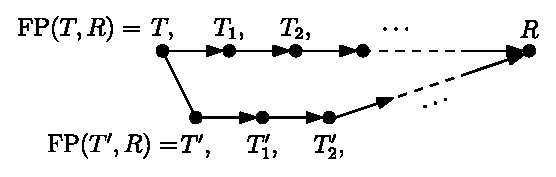
\includegraphics[width=0.6\textwidth]{proof_idea_ag}
\caption{Trees $T$, $T'$, and $R$ as in inequality~(\ref{eqn:iff_inequality}).
Paths $\fp(T,R) = [T,T_1,T_2, \ldots, R]$ and $\fp(T',R) = [T',T'_1,T'_2, \ldots, R]$ are indicated by arrows.}
\label{fig:proof_idea}
\end{figure}

Assume to the contrary that $T$ and $R$ are trees for which there exists $T'$ violating inequality~(\ref{eqn:iff_inequality}).
Out of all such pairs $T, R$ choose one with the minimal $|\fp(T, R)|$.
Denote $\fp(T,R) = [T, T_1, T_2, \ldots, R]$ and $\fp(T', R) = [T', T_1', T_2', \ldots, R]$, and let $[(T)_t, (T)_{t+1}]$ be the interval in $T$ on which the $\rnni$ move connecting $T$ and $T'$ is performed.
Let $C_k$ be the cluster of $R$ such that the node $(C_k)_T$ is moved down by the first move on $p$.
If the rank of $(C_k)_T$ is not in $\{t, t+1\}$ then $(C_k)_T$ and $(C_k)_{T'}$ induce the same cluster, so $\findpath$ would make the same rearrangement in both trees $T$ and $T'$ in the first move along $\fp(T, R)$ and $\fp(T', R)$ resulting in trees $T_1$ and $T_1'$ which are $\rnni$ neighbours, as in Figure~\ref{fig:proof_idea}.
In this case, paths $\fp(T_1, R)$ and $\fp(T_1', R)$ violate inequality~(\ref{eqn:iff_inequality}) but $\fp(T_1, R)$ is strictly shorter than $\fp(T, R)$, contradicting our minimality assumption.
Hence, the first move on $p$ has to involve an interval incident to at least one of the nodes $(T)_t$, $(T)_{t+1}$.

We will distinguish two cases depending on whether $T$ and $T'$ are connected by an $\nni$ or a rank move.
For each of these we will further distinguish all possible moves between $T$ and $T_1$.

\textbf{Case 1.}
$T$ and $T'$ are connected by an $\nni$ move, so $((T)_t,(T)_{t+1})$ is an edge in $T$ -- see Figure~\ref{fig:thm_fp_nni1}.
Denote the clusters induced by the children of $(T)_t$ by $A$ and $B$ and the cluster induced by the child of $(T)_{t+1}$ that is not $(T)_t$ by $C$, and assume that the $\nni$ move between $T$ and $T'$ exchanges the subtrees induced by clusters $B$ and $C$.
Additionally, denote the cluster induced by the child of $(T)_{t+2}$ that is not $(T)_{t+1}$ by $D$ -- see Figure~\ref{fig:thm_fp_nni2a}.

\begin{figure}[!hbt]
\centering
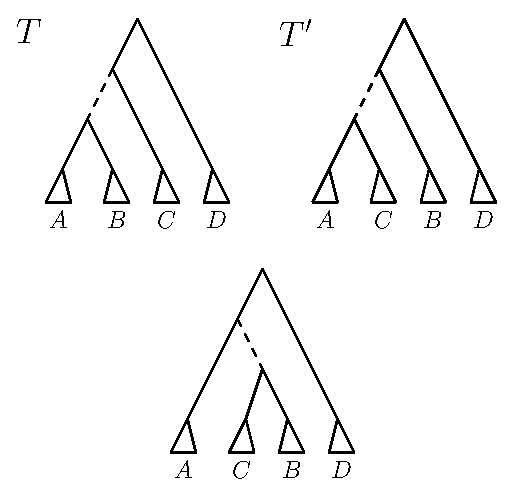
\includegraphics[width=0.35\textwidth]{thm_fp_nni1}
\caption{$\nni$ move between $T$ and $T'$ on the bold edge $((T)_t,(T)_{t+1})$ and the third $\rnni$ neighbour resulting from a move on that edge.}
\label{fig:thm_fp_nni1}
\end{figure}

We now consider all possible moves $\findpath$ can perform to go from $T$ to $T_1$ that involve a node of rank $t$ or $t+1$, that is, we will consider three intervals in total.

\begin{enumerate}[label = 1.{\arabic*}]
\item $\rnni$ move on interval $[(T)_t, (T)_{t+1}]$.
Note that this move has to be the $\nni$ move that is different from the $\nni$ move connecting $T$ and $T'$.

In this case, the cluster $B \cup C$ is built in $T_1$, as depicted in the bottom of Figure~\ref{fig:thm_fp_nni1}.
It follows that the cluster $C_k$ that is considered first by $\findpath$ must contain taxa from both $B$ and $C$.
But then $\findpath$ applied to $T'$ and $R$ has to decrease the rank of $(C_k)_{T'}$ in its first step implying that $T'_1 = T_1$, so $|\fp(T',R)| = |\fp(T,R)|$.
This contradicts our assumption that $|\fp(T',R)| < |\fp(T,R)| - 1$.

\item $\nni$ move on (edge) interval $[(T)_{t+1}, (T)_{t+2}]$ that swaps the subtrees induced by clusters $C$ and $D$.
This move is shown in Figure~\ref{fig:thm_fp_nni2a} by an arrow from $T$ to the leftmost tree in the middle row.

\begin{figure}[H]
	\begin{subfigure}[b]{.45\textwidth}
		\centering
		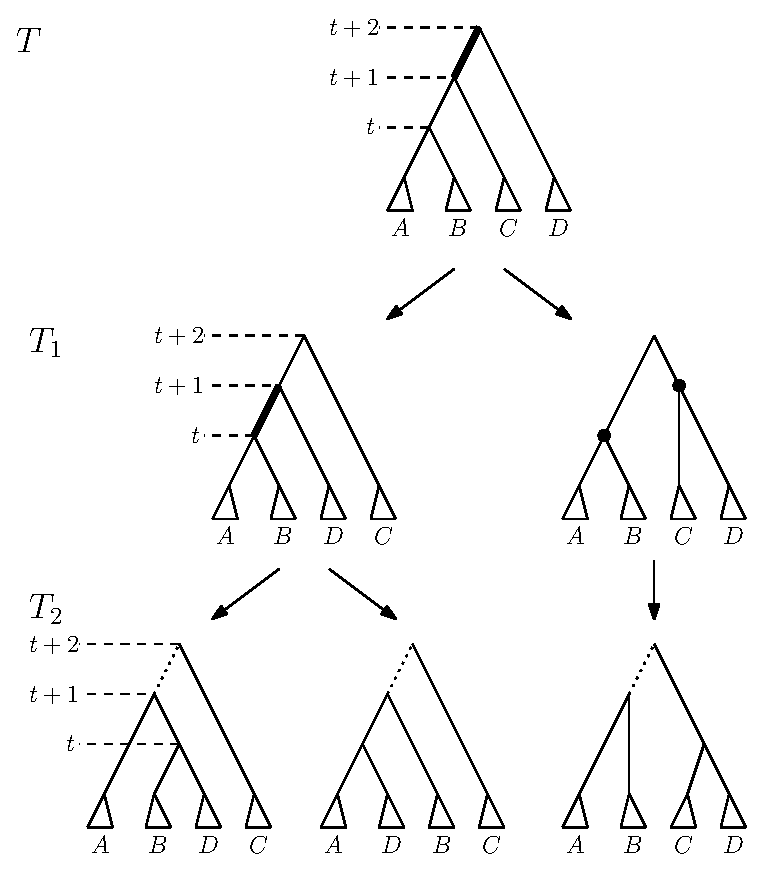
\includegraphics[width=0.9\linewidth]{thm_fp_nni2a.eps}
		\vspace{12pt}
		\caption{Possible initial segments of $\fp(T, R)$}
		\label{fig:thm_fp_nni2a}
	\end{subfigure}
	\begin{subfigure}[b]{.45\textwidth}
		\centering
		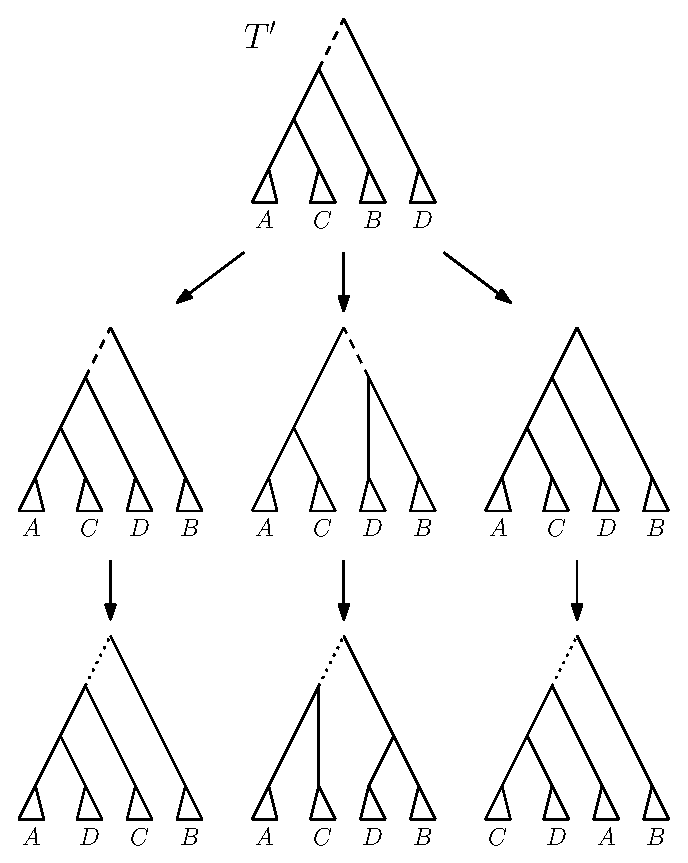
\includegraphics[width=0.9\linewidth]{thm_fp_nni2b.eps}
		\vspace{12pt}
		\caption{Possible initial segments of $\fp(T', R)$}
		\label{fig:thm_fp_nni2b}
	\end{subfigure}
	\caption{Comparison of paths $\fp(T, R)$ and $\fp(T', R)$ if $T$ and $T'$ are connected by an $\nni$ move on edge $((T)_{t+1},T_{t+2})$ in $T$.
	The bottom row displays all possibilities for $T_2$ and $T'_2$, depending on the position of cluster $C_k$ that is considered by $\findpath$:
	${C_k \subseteq B \cup D}$ is on the left, ${C_k \subseteq A \cup D}$ is in the middle, ${C_k \subseteq C \cup D}$ is on the right.
	Since the position of the tree root is irrelevant, so we have placed the root to simplify the figures.}
	\label{fig:thm_fp_nni}
\end{figure}

Note that the cluster $C_k$ that is considered by $\findpath$ in the first step of computing $\fp(T, R)$ must intersect $D$.
Additionally, $C_k$ must intersect $A$, or $B$, or both of them.
Hence, we will consider each of these three cases individually.
We can assume that $k > 1$ and $C_{k-1} = (R)_{k-1}$.
\todo{We need to clarify this. LC: what exactly needs to be clarified here?}
Indeed, $C_1 \subseteq A \cup D$ or $C_1 \subseteq B \cup D$.

We will use Figure~\ref{fig:thm_fp_nni} to demonstrate all the three cases below.

\begin{enumerate}[label = \theenumi.\arabic*]
\item $C_k$ intersects each of $A$, $B$, and $D$.
Since $C_k$ is the first cluster considered by $\findpath$, the two clusters that make up $C_k$ in $R$ must be present in $T$.
So $C_{k-1} = A \cup B$.
Since $A \cup B$ is not a cluster in $T'$, $\findpath$ will decrease the rank of $(C_{k-1})_{T'}$ on $\fp(T', R)$ before considering cluster $C_k$.
\todo{How do we know the algorithm doesn't have to consider $C_i$s for $i < k-1$?}
This $\rnni$ move decreases the rank of $(C_{k-1})_{T'}$ by building cluster $A \cup B$, in which case $T'_1 = T$.
This however contradicts to $|\fp(T',R)| < |\fp(T,R)| - 1$.

\item $C_k \subseteq A \cup D$.
\label{deep_case_details}
Starting from $T$, $\findpath$ exchanges first subtrees induced by clusters $C$ and $D$ and then by $B$ and $D$.
This results in trees $T_1$ and $T_2$ -- see the path leading to the tree in the middle of the bottom row in Figure~\ref{fig:thm_fp_nni2a}.
Starting from $T'$, $\findpath$ exchanges first subtrees induced by $B$ and $D$ and then by $C$ and $D$.
This results in trees $T_1'$ and $T_2'$ -- see the path leading to the tree in the middle of the bottom row in Figure~\ref{fig:thm_fp_nni2b}.
It follows that $T_2$ and $T'_2$ only differ by one interval (indicated by dotted edges in the corresponding trees in Figure~\ref{fig:thm_fp_nni}), and hence they are $\rnni$ neighbours.
This together with the facts that $|\fp(T_2,R)| = |\fp(T,R)|-2$ and $|\fp(T'_2,R)| = |\fp(T',R)|-2$ contradicts the assumption that $|\fp(T,R)|$ is a minimal length violating inequality~(\ref{eqn:iff_inequality}).

\item $C_k \subseteq B \cup D$.
This case is analogous to the previous one.
The two initial segments of $\fp(T, R)$ and $\fp(T', R)$ are the paths leading to the leftmost trees in the bottom row of Figures~\ref{fig:thm_fp_nni2a} and \ref{fig:thm_fp_nni2b}, respectively.
Note that the rank swap leading from $T_1'$ to $T_2'$ is required because the rank of $(C_k)_R$ is at most $t$ as implied by the move leading from $T_1$ to $T_2$.
The corresponding trees $T_2$ and $T_2'$ are again $\rnni$ neighbours.
\end{enumerate}

\item $\nni$ move on (edge) interval $[(T)_{t+1}, (T)_{t+2}]$ that builds a cluster $C \cup D$ in $T_1$.
\label{case:one_or_two_moves_down}
This move is shown in Figure~\ref{fig:thm_fp_nni2a} by an arrow from $T$ to the second leftmost tree in the middle row.
In this case, $C_k \subseteq C \cup D$.

If the ranks of $(C_k)_{T_1}$ and $(C_k)_R$ coincide then $C_{k-1} = A \cup B$ is a cluster in $R$.
Since $A \cup B$ is not a cluster in $T'$, the first $\rnni$ move on $\fp(T', R)$ builds the cluster $A \cup B$ by swapping subtrees induced by cluster $B$ and $C$.
This move results in $T_1' = T$ contradicting $|\fp(T',R)| < |\fp(T,R)| - 1$.

If the rank of $(C_k)_{T_1}$ is strictly higher than that of $(C_k)_R$ then $\findpath$ decreases the rank of $(C_k)_{T_1}$ in the second step.
This results in the path from $T$ to the rightmost tree in Figure~\ref{fig:thm_fp_nni2a}.
Hence, $\fp(T', R)$ has to also begin with two moves that decrease the rank of $(C_k)_{T'}$ twice, resulting in the rightmost path in Figure~\ref{fig:thm_fp_nni2b}.
Similarly to case~\ref{deep_case_details}, we arrive at a contradiction that trees $T_2$, $T_2'$, and $R$ violate inequality~(\ref{eqn:iff_inequality}) and $|\fp(T_2,R)| < |\fp(T,R)|$.

\item Rank move on interval $[(T)_{t+1},(T)_{t+2}]$.
This case is analogous to case~\ref{case:one_or_two_moves_down}.
If the ranks of $(C_k)_{T_1}$ and $(C_k)_R$ coincide then $C_{k-1} = A \cup B$ is a cluster in $R$, and applying $\findpath$ to $T', R$ we get $T'_1 = T$.
If the rank of $(C_k)_{T_1}$ is strictly higher than that of $(C_k)_R$ then $\findpath$ decreases the rank of $(C_k)_{T_1}$ in the second step.
Recall that the interval between nodes of rank $t$ and $t+1$ is an edge in both $T$ and $T'$.
Hence, the first two moves on $\fp(T', R)$ decrease the rank of $(C_k)_{T'}$ twice resulting in $T'_2$ which is an $\rnni$ neighbour of $T_2$.
As before, this contradicts our minimality assumption.

\item $\rnni$ move on interval $[(T)_{t-1},(T)_t]$.
In this case $C_k \subseteq A \cup B$, so the first move on $\fp(T', R)$ decreases the rank of $(C_k)_{T'}$ by exchanging the subtrees induced by $B$ and $C$.
This results in $T'_1 = T$.
This argument applies whether or not $((T)_{t-1},(T)_t)$ is an edge in $T$.
\end{enumerate}

\textbf{Case 2.}
$T$ and $T'$ are connected by a rank move on the interval between nodes or rank $t$ and $t+1$.
Denote the cluster induced by $(T)_t$ by $A$, the clusters induces by the children of $(T)_t$ by $A_1$ and $A_2$, the cluster induced by $(T)_{t+1}$ by $B$, and the cluster induced by the children of $(T)_{t+1}$ by $B_1$ and $B_2$ -- see Figure~\ref{fig:thm_fp_rank1}.

\begin{figure}[!hbt]
\centering
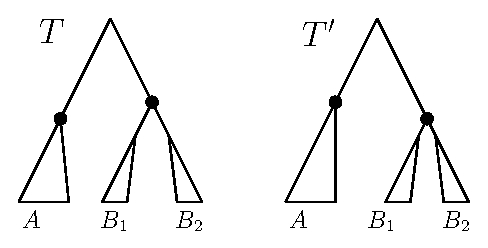
\includegraphics[width=0.4\textwidth]{thm_fp_rank1}
\caption{Rank move between $T$ and $T'$ on the interval above the node of rank $t$, and possible initial segments of $\fp(T, R)$ and $\fp(T', R)$.
We use notations $A = A_1 \cup A_2$ and $B = B_1 \cup B_2$.}
\label{fig:thm_fp_rank1}
\end{figure}

We again consider all possible moves $\findpath$ can perform to go from $T$ to $T_1$ that involve a node of rank $t$ or $t+1$.

\begin{enumerate}[label = 2.\arabic*]
\item Rank move on $[(T)_t,(T)_{t+1}]$.
This move results in $T_1 = T'$.

\item $\nni$ move on (edge) interval $[(T)_{t+1},(T)_{t+2}]$.
The following two sub-cases are analogous to case~\ref{case:one_or_two_moves_down}.

\begin{enumerate}[label = \theenumi.\arabic*]
	\item $(T)_{t+2}$ is a parent of $(T)_t$.
	The first move on $\fp(T, R)$ builds a cluster $A \cup B_1$ or $A \cup B_2$, and we assume without loss of generality that it is the former, as in Figure~\ref{fig:thm_fp_rank1}.
	This implies that $C_k \subseteq A \cup B_1$.
	If the ranks of $(C_k)_{T_1}$ and $(C_k)_R$ coincide then $C_{k-1} = A$ is a cluster in $R$.
	Therefore, the first move on $\fp(T', R)$ decreases the rank of $(A)_{T'}$, which results in $T_1' = T$.
	If the rank of $(C_k)_{T_1}$ is strictly higher than that of $(C_k)_R$ then $\findpath$ decreases the rank of $(C_k)_{T_1}$ in the second step.
	Due to the symmetry we can assume that $C_k \subseteq A_1 \cup B_1$, which implies that the move between $T_1$ to $T_2$ exchanges the subtrees induced by $A_2$ and $B_1$, as depicted on the left of Figure~\ref{fig:thm_fp_rank1}.
	$C_k \subseteq A_1 \cup B_1$ implies that the first two moves on $\fp(T', R)$ result in a tree $T'_2$ that is an $\rnni$ neighbour of $T_2$ -- see Figure~\ref{fig:thm_fp_rank1}.
	This is a contradiction to the minimality assumption on $|\fp(T,R)|$.

	\item $(T)_{t+2}$ is not a parent of $(T)_t$.
	In this case, there exists a cluster $C$ induced by the child of $(T)_{t+2}$ which is different from the one that induces $B$ -- see Figure~\ref{fig:thm_fp_rank2}.
\begin{figure}[!hbt]
	\centering
	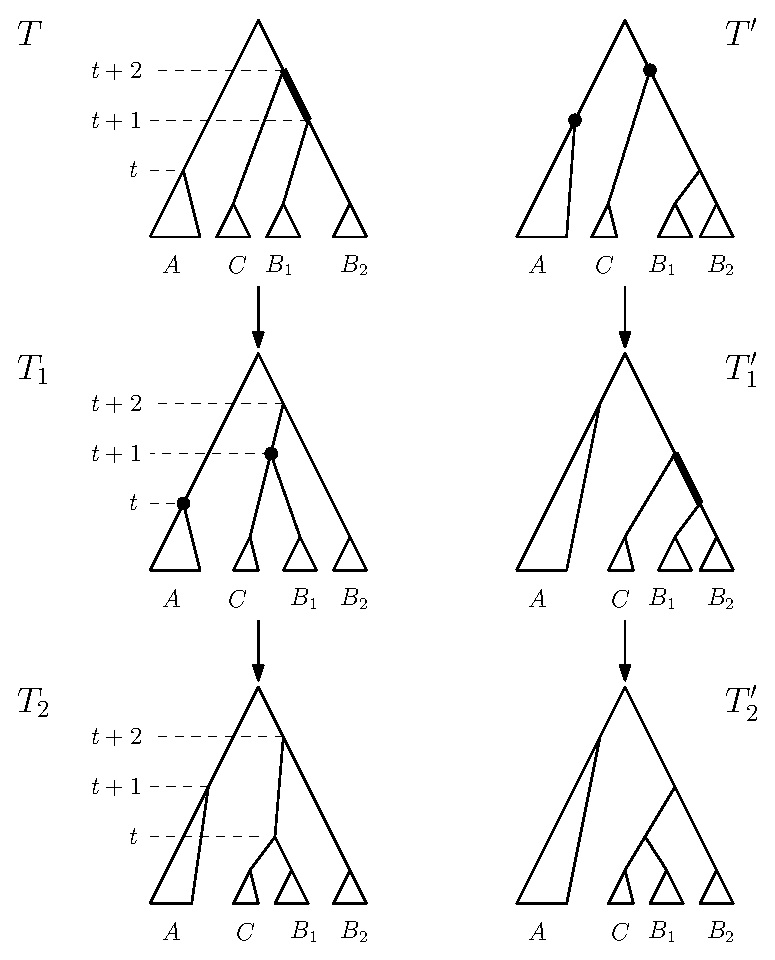
\includegraphics[width=0.4\textwidth]{thm_fp_rank2}
	\caption{Comparison of $p$ (left) and $p'$ (right) if there is a rank move between $T$ and $T'$ and an $\nni$ move on the edge below the corresponding (rank) interval follows on $p$.}
	\label{fig:thm_fp_rank2}
\end{figure}
	We can assume without loss of generality that $C_k \subseteq C \cup B_1$ and the first move on $\fp(T, R)$ builds a new cluster $C \cup B_1$.
	If the ranks of $(C_k)_{T_1}$ and $(C_k)_R$ coincide then $C_{k-1} = A$ is a cluster in $R$, which implies that $A$ is induced by the node of rank $t$ in both $T$ and $R$.
	So $T'_1 = T$.
	If the rank of $(C_k)_{T_1}$ is strictly higher than that of $(C_k)_R$ then $\findpath$ decreases the rank of $(C_k)_{T_1}$ in the second step -- see Figure~\ref{fig:thm_fp_rank2}.
	The corresponding first moves on $\fp(T', R)$ are shown on the right in Figure~\ref{fig:thm_fp_rank2}, and we again get that $T_2$ and $T_2'$ are $\rnni$ neighbours.
\end{enumerate}

\item Rank move on interval $[(T)_{t+1}, (T)_{t+2}]$.
Again, depending on whether or not the ranks of $(C_k)_{T_1}$ and $(C_k)_R$ coincide, we arrive at the conclusion that either $T_1' = T$ or $T_2$ and $T_2'$ are $\rnni$ neighbours.

\item $\rnni$ move on interval $[(T)_{t-1},(T)_t]$.
In this case $C_k \subseteq A$ and the first move on $\fp(T', R)$ must be a rank swap resulting in $T_1' = T$.
\end{enumerate}

Since all possible cases result in a contradiction, we conclude that inequality~(\ref{eqn:iff_inequality}) is true for all trees, which completes the proof of the theorem.
\endproof

\end{document}
